% !Mode:: "TeX:UTF-8"
% Author: Zhengxi Tian
% Email: zhengxi.tian@hotmail.com

\chapter{不同模型的系统得分}\label{ch:model_system_dist}
我们在这里展示了不同模型的不同指标的箱体图。
横坐标是模型,每一个箱子概括了三个数据集的情况。
箱子的上面和下面的黑线是模型得分的标准差,表示得分的变动范围。
从这些图像我们可以清楚的看到模型在数据集上的平均水平以及模型得分的相对高低。
这些图像从模型的维度再现了第~\ref{sec:system_scores}~节的结论。
但是,由于数据集对指标得分的影响大于模型,一个模型在多个数据集上的分布
有较大的方差。

% -- Boxplot Model -- %
\begin{figure}[H]
    \begin{subfigure}{0.5\linewidth}
        \centering
        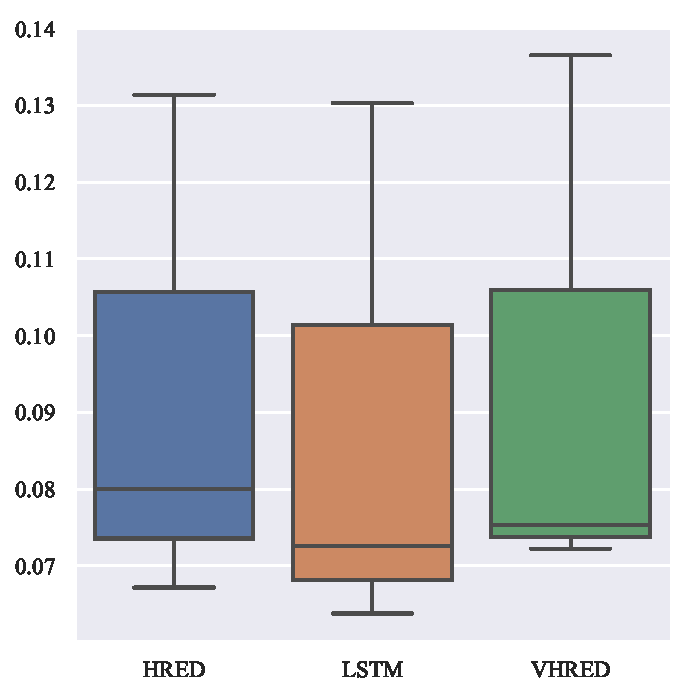
\includegraphics[width=\linewidth]{figure/boxplot/model/bleu_1/plot.pdf}
        \caption{BLEU-1}
    \end{subfigure}%
    \begin{subfigure}{0.5\linewidth}
        \centering
        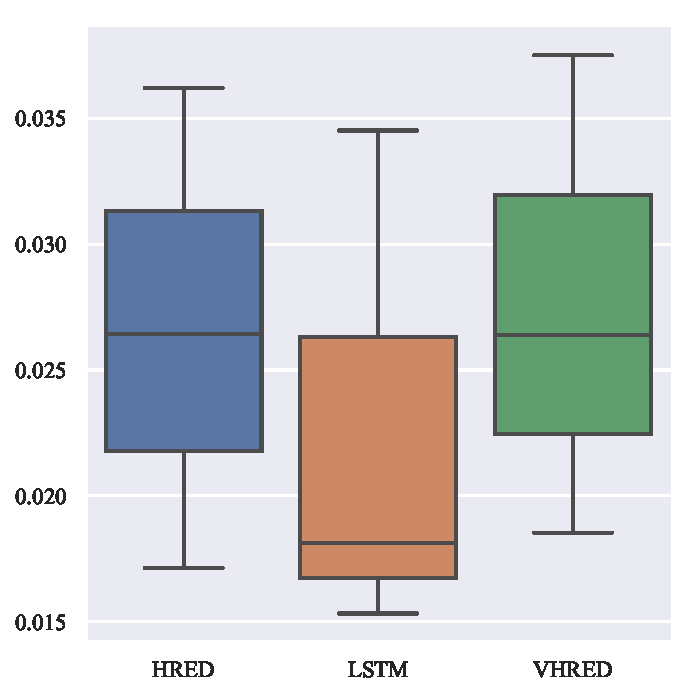
\includegraphics[width=\linewidth]{figure/boxplot/model/bleu_2/plot.pdf}
        \caption{BLEU-2}
    \end{subfigure}
    \begin{subfigure}{0.5\linewidth}
        \centering
        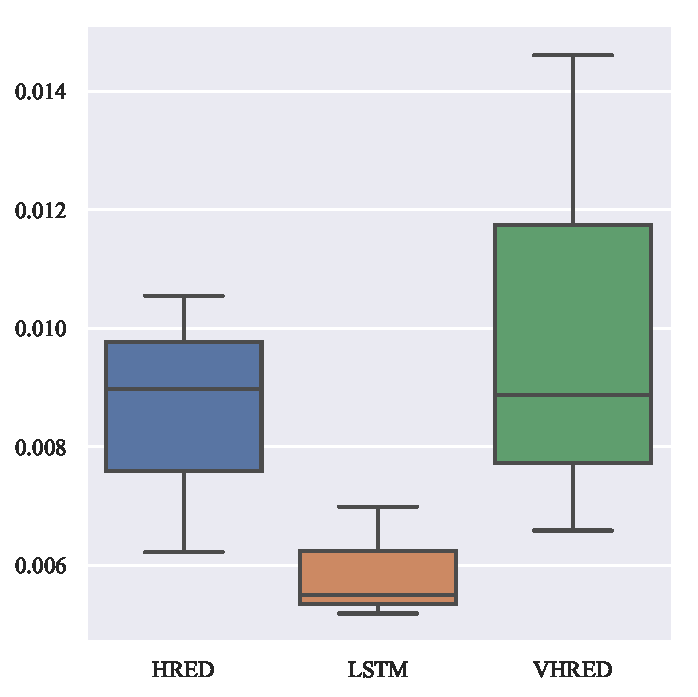
\includegraphics[width=\linewidth]{figure/boxplot/model/bleu_3/plot.pdf}
        \caption{BLEU-3}
    \end{subfigure}%
    \begin{subfigure}{0.5\linewidth}
        \centering
        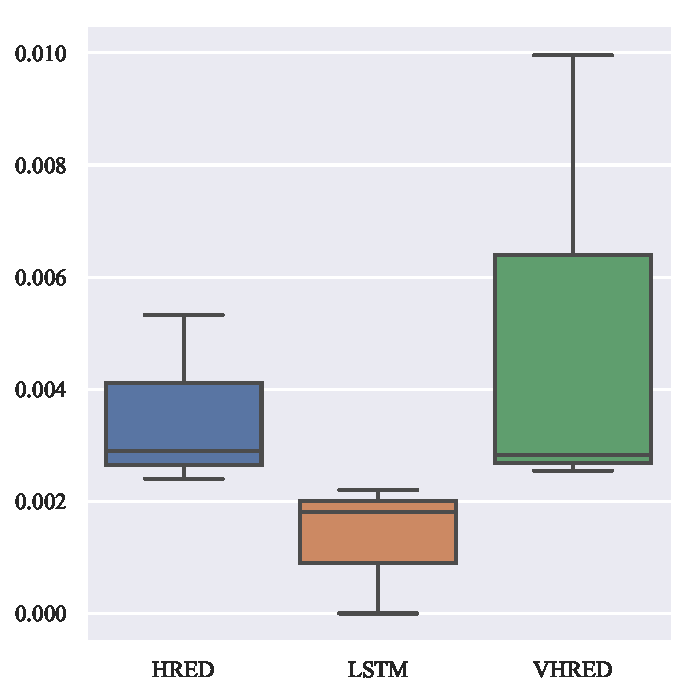
\includegraphics[width=\linewidth]{figure/boxplot/model/bleu_4/plot.pdf}
        \caption{BLEU-4}
    \end{subfigure}
    \centering
    \caption{不同模型的BLEU分布}
    \label{fig:BLEU_model}
\end{figure}

\begin{figure}[H]
    \begin{subfigure}{0.5\linewidth}
        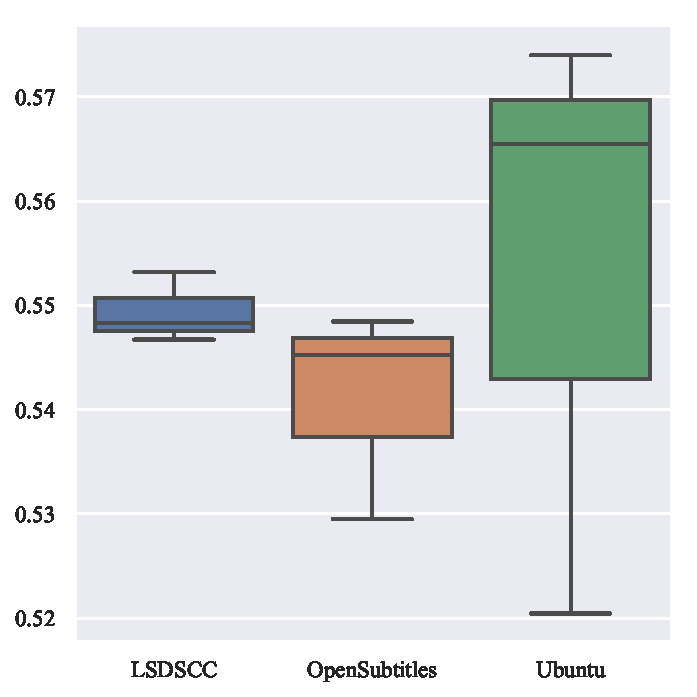
\includegraphics[width=\linewidth]{figure/boxplot/dataset/embedding_based_vector_average/plot.pdf}
        \centering
        \caption{Average}
    \end{subfigure}%
    \begin{subfigure}{0.5\linewidth}
        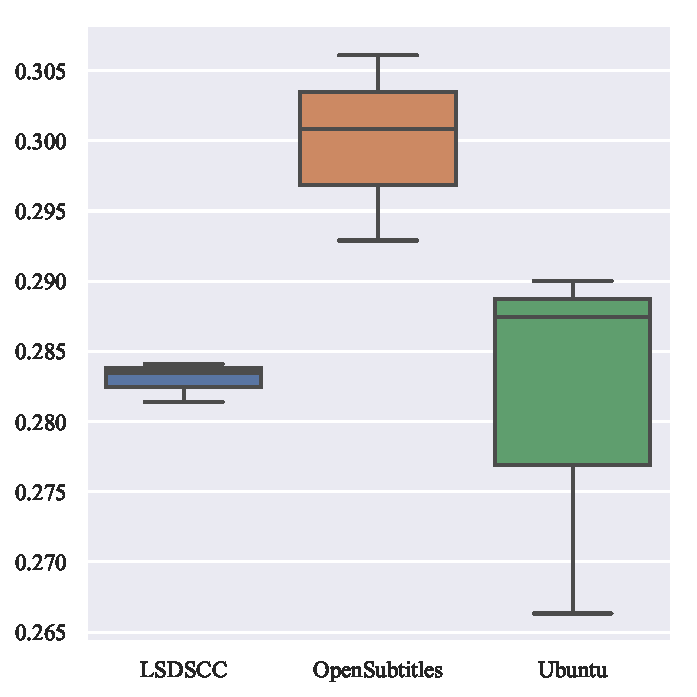
\includegraphics[width=\linewidth]{figure/boxplot/dataset/embedding_based_vector_extrema/plot.pdf}
        \centering
        \caption{Extrema}
    \end{subfigure}
    \begin{subfigure}{0.5\linewidth}
        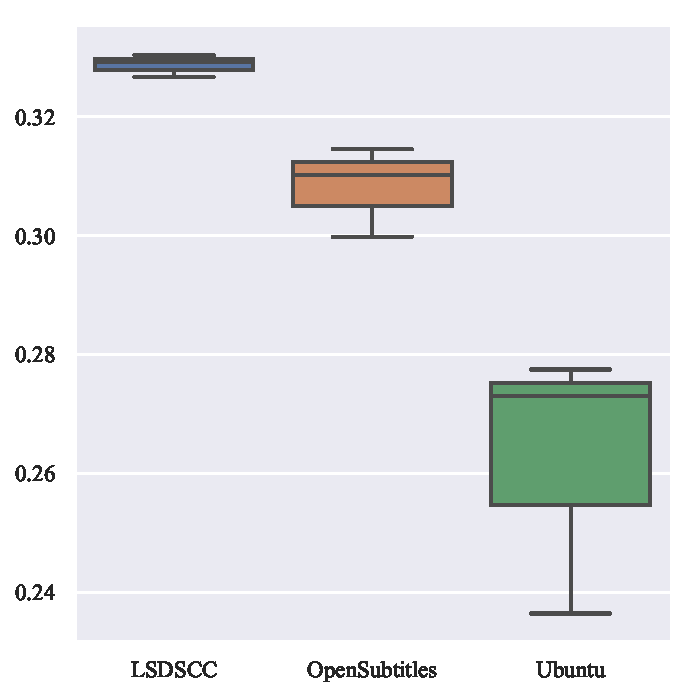
\includegraphics[width=\linewidth]{figure/boxplot/dataset/embedding_based_greedy_matching/plot.pdf}
        \centering
        \caption{Greedy}
    \end{subfigure}%
    \begin{subfigure}{0.5\linewidth}
        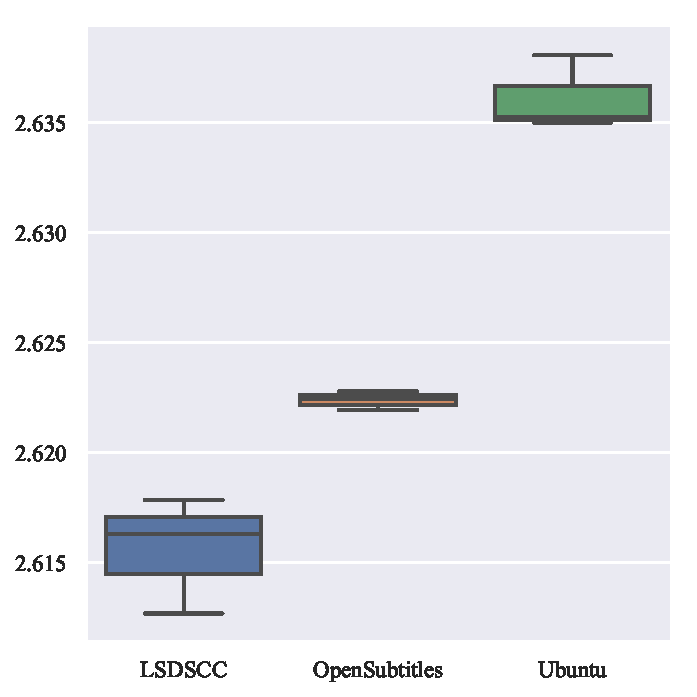
\includegraphics[width=\linewidth]{figure/boxplot/dataset/adem/plot.pdf}
        \centering
        \caption{ADEM}
        \label{subfig:ADEM_system}
    \end{subfigure}
    \caption{基于词嵌入的指标和ADEM的系统得分}
    \label{fig:ADEM_EB_system}
\end{figure}

\begin{figure}[H]
    \begin{subfigure}{0.5\linewidth}
        \centering
        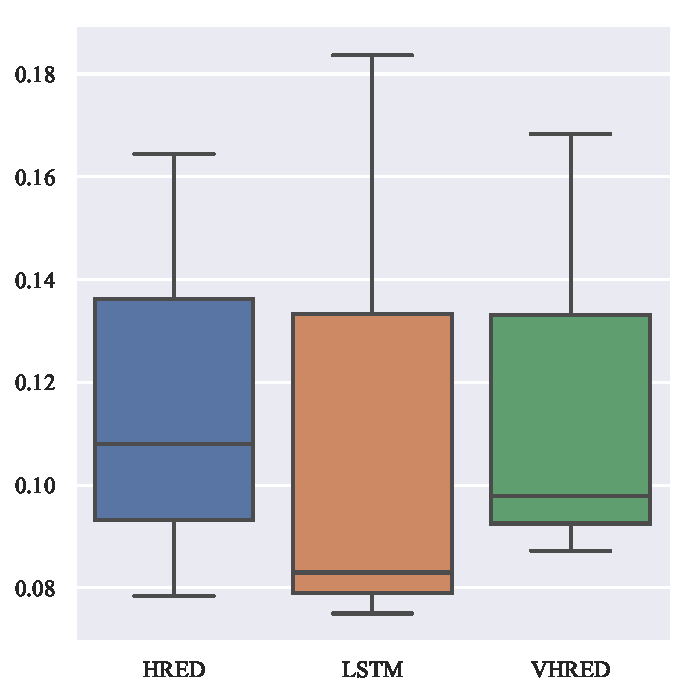
\includegraphics[width=\linewidth]{figure/boxplot/model/rouge_1/plot.pdf}
        \caption{ROUGE-1}
    \end{subfigure}%
    \begin{subfigure}{0.5\linewidth}
        \centering
        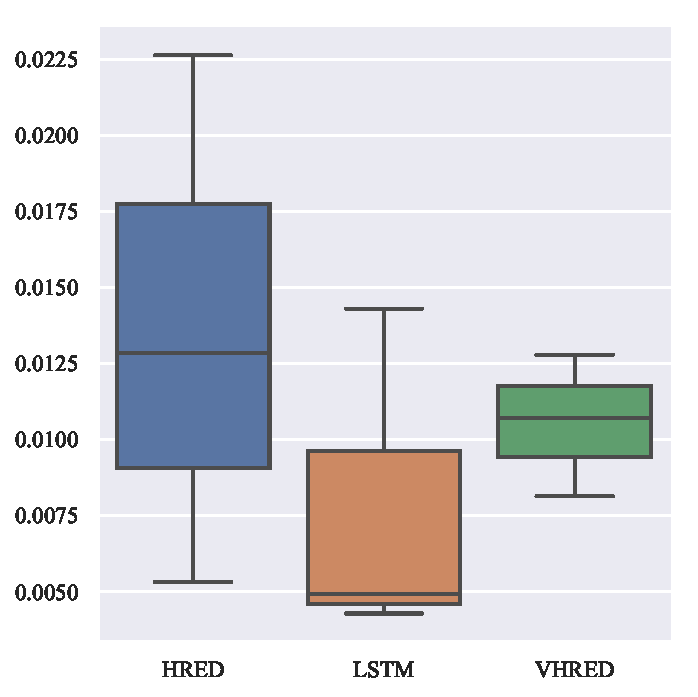
\includegraphics[width=\linewidth]{figure/boxplot/model/rouge_2/plot.pdf}
        \caption{ROUGE-2}
    \end{subfigure}
    \begin{subfigure}{0.5\linewidth}
        \centering
        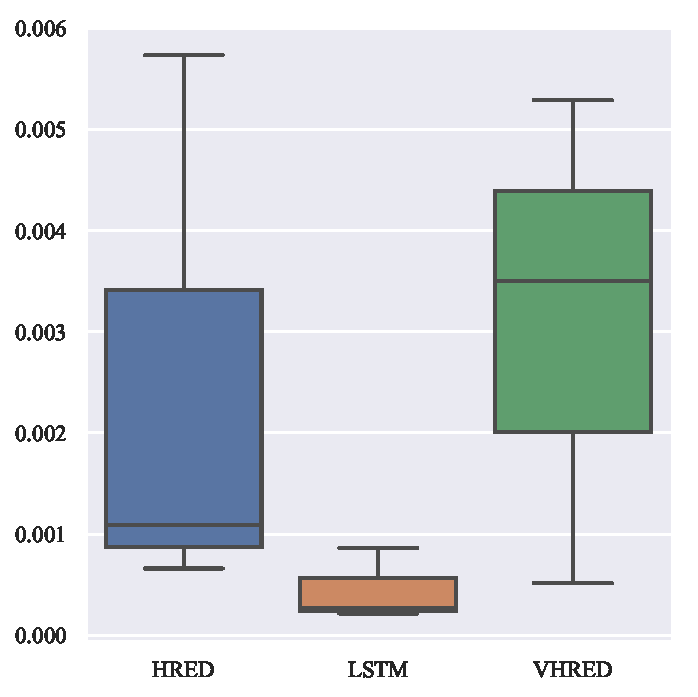
\includegraphics[width=\linewidth]{figure/boxplot/model/rouge_3/plot.pdf}
        \caption{ROUGE-3}
    \end{subfigure}%
    \begin{subfigure}{0.5\linewidth}
        \centering
        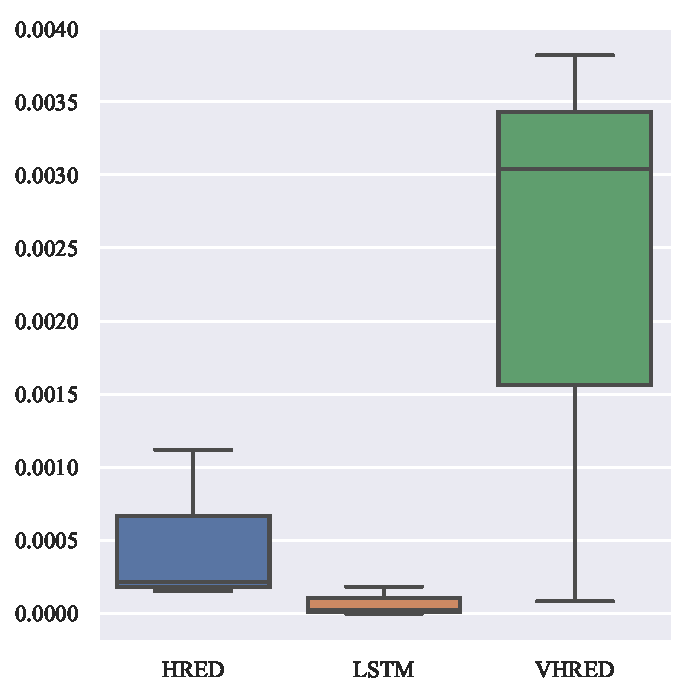
\includegraphics[width=\linewidth]{figure/boxplot/model/rouge_4/plot.pdf}
        \caption{ROUGE-4}
    \end{subfigure}
    \centering
    \caption{不同模型的ROUGE-N分布}
    \label{fig:ROUGE_N_model}
\end{figure}
\begin{figure}[H]
    \begin{subfigure}{0.5\linewidth}
        \centering
        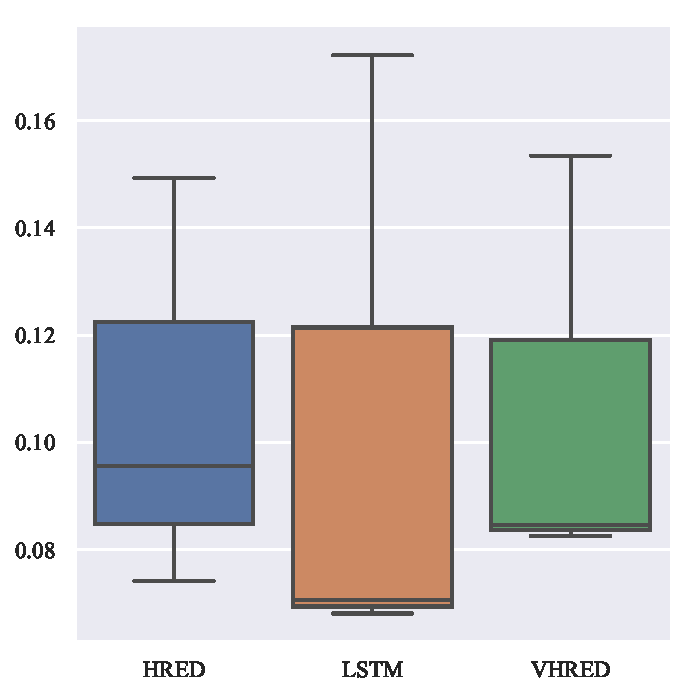
\includegraphics[width=\linewidth]{figure/boxplot/model/rouge_l/plot.pdf}
        \caption{ROUGE-L}
    \end{subfigure}%
    \begin{subfigure}{0.5\linewidth}
        \centering
        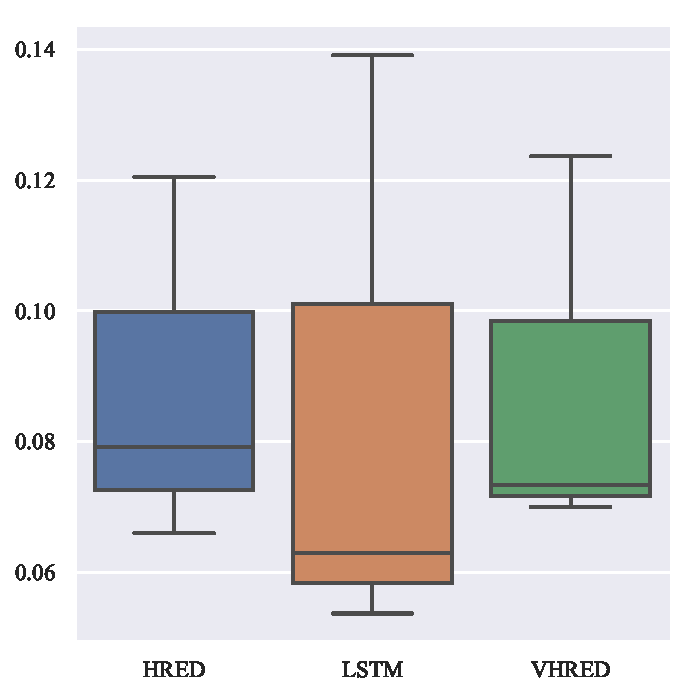
\includegraphics[width=\linewidth]{figure/boxplot/model/rouge_w/plot.pdf}
        \caption{ROUGE-W}
    \end{subfigure}
    \centering
    \caption{不同模型的ROUGE-L和ROUGE-W分布}
    \label{fig:ROUGE_LW_model}
\end{figure}

\begin{figure}[H]
    \begin{subfigure}{0.5\linewidth}
        \centering
        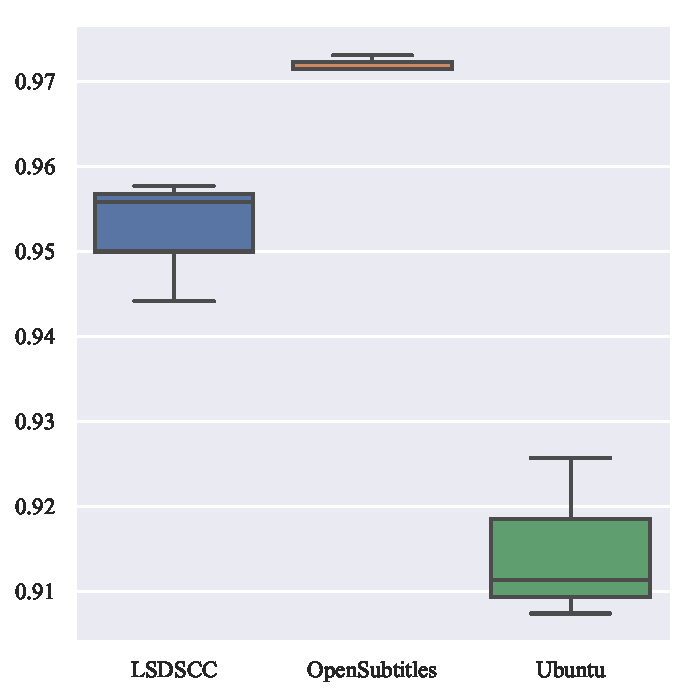
\includegraphics[width=\linewidth]{figure/boxplot/dataset/distinct_1/plot.pdf}
        \caption{Distinct-1}
        \label{fig:distinct_1_system}
    \end{subfigure}%
    \begin{subfigure}{0.5\linewidth}
        \centering
        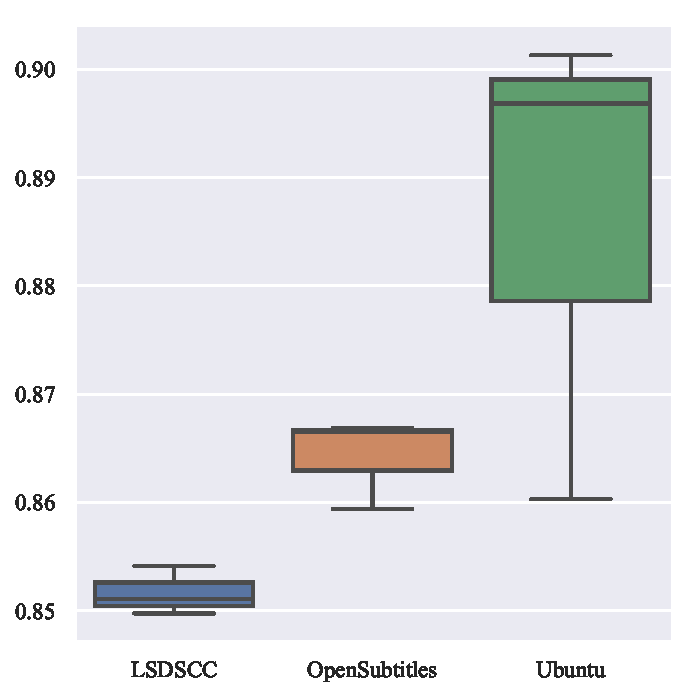
\includegraphics[width=\linewidth]{figure/boxplot/dataset/distinct_2/plot.pdf}
        \caption{Distinct-2}
        \label{fig:distinct_2_system}
    \end{subfigure}

    \begin{subfigure}{0.5\linewidth}
        \centering
        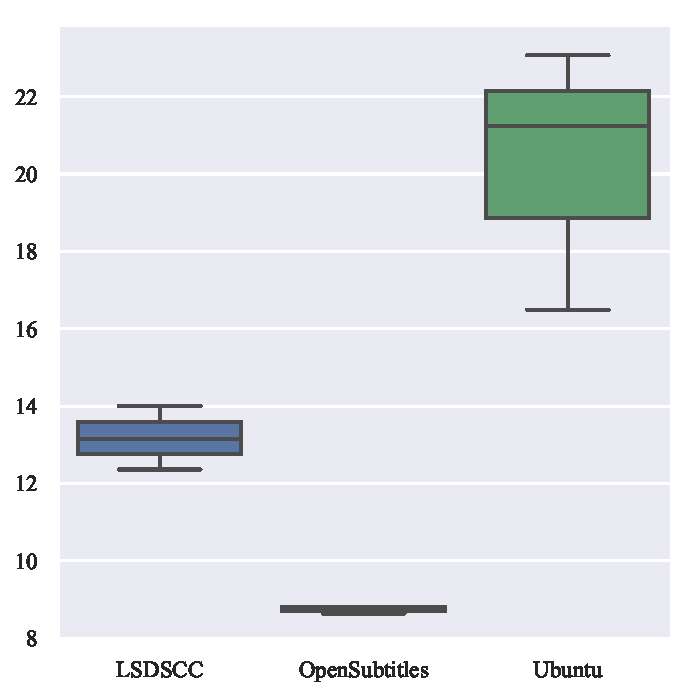
\includegraphics[width=\linewidth]{figure/boxplot/dataset/utterance_len/plot.pdf}
        \caption{\#words}
        \label{fig:words_system}
    \end{subfigure}%
    \begin{subfigure}{0.5\linewidth}
        \centering
        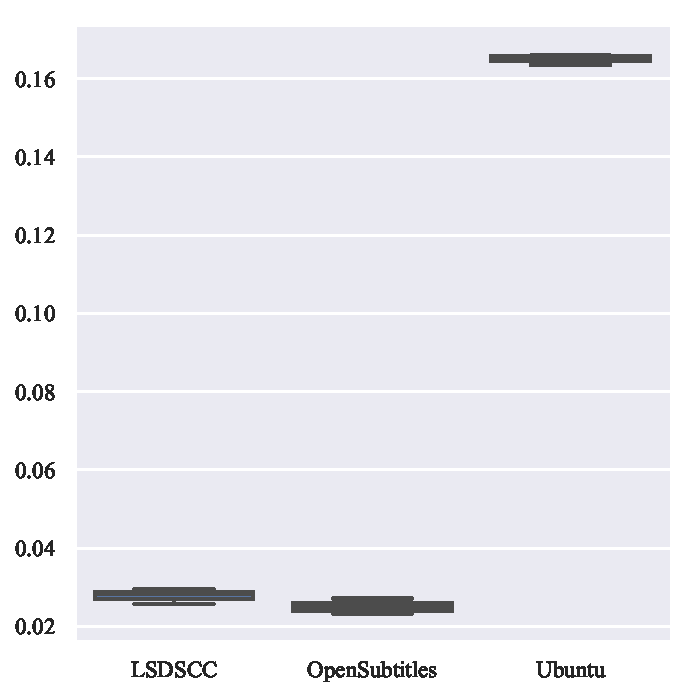
\includegraphics[width=\linewidth]{figure/boxplot/dataset/meteor/plot.pdf}
        \caption{METEOR}
        \label{fig:meteor_system}
    \end{subfigure}
    \caption{Distinct-N,\#words和METEOR的系统得分}
    \label{fig:Other_system}
\end{figure}

